\documentclass[tikz,border=0pt]{standalone}
% Shared TikZ style for figures in
% Layered Network Programming with SNode.C.
%
% Contract for this figure set:
% - every figure PDF has an exact 160 mm canvas width;
% - the TikZ drawing is rendered at native size, not scaled;
% - the drawing is horizontally centered on that canvas;
% - semantic colors, line widths, arrow widths, boundary titles, and spacing
%   are kept consistent unless a local exception is needed to fit the canvas.

\usepackage{xcolor}
\usepackage{tikz}
\usetikzlibrary{
  arrows.meta,
  backgrounds,
  calc,
  fit,
  matrix,
  positioning,
  shapes.geometric,
  shapes.multipart
}

% ----------------------------------------------------------------------
% Palette.
% ----------------------------------------------------------------------
\definecolor{snodecInk}{HTML}{17212B}
\definecolor{snodecMuted}{HTML}{4B5F68}
\definecolor{snodecRule}{HTML}{7A8B93}

\definecolor{snodecBlue}{HTML}{0B4F6C}
\definecolor{snodecBlueSoft}{HTML}{E3F2F8}

\definecolor{snodecGreen}{HTML}{1F7A68}
\definecolor{snodecGreenSoft}{HTML}{E5F4EF}

\definecolor{snodecOrange}{HTML}{C46A1B}
\definecolor{snodecOrangeSoft}{HTML}{FAEFE3}

\definecolor{snodecRed}{HTML}{B24A4A}
\definecolor{snodecRedSoft}{HTML}{F8E8E8}

\definecolor{snodecGraySoft}{HTML}{F1F3F2}

% Title-color palette:
% same hue family as the box, but with stronger contrast.
\colorlet{snodecTitleBlue}{snodecBlue}
\definecolor{snodecTitleGreen}{HTML}{155F51}
\definecolor{snodecTitleOrange}{HTML}{A95516}
\definecolor{snodecTitleGray}{HTML}{4B5F68}
\colorlet{snodecTitleRed}{snodecRed}

% ----------------------------------------------------------------------
% Geometry and line constants.
% ----------------------------------------------------------------------
\newcommand{\snodecCanvasHalfWidth}{80mm}
\newcommand{\snodecCanvasVMargin}{7pt}

\newcommand{\snodecBoxCorner}{2.5pt}
\newcommand{\snodecBoundaryCorner}{3pt}

\newcommand{\snodecBoxLineWidth}{0.70pt}
\newcommand{\snodecInnerLineWidth}{0.58pt}
\newcommand{\snodecBoundaryLineWidth}{0.58pt}
\newcommand{\snodecArrowLineWidth}{0.70pt}
\newcommand{\snodecSecondaryLineWidth}{0.58pt}
\newcommand{\snodecBusLineWidth}{0.58pt}

\newcommand{\snodecBoxXSep}{3mm}
\newcommand{\snodecBoxYSep}{2.5mm}
\newcommand{\snodecSmallBoxXSep}{1.2mm}
\newcommand{\snodecSmallBoxYSep}{1.6mm}
\newcommand{\snodecBoundaryInnerSep}{4.5mm}

\newcommand{\snodecGapSmall}{6mm}
\newcommand{\snodecGapNormal}{8mm}
\newcommand{\snodecGapLarge}{11mm}
\newcommand{\snodecGapMajor}{14mm}
\newcommand{\snodecBendLeg}{6mm}
\newcommand{\snodecOutsideLane}{8mm}

% ----------------------------------------------------------------------
% Shared TikZ styles.
% ----------------------------------------------------------------------
\tikzset{
  snodec diagram/.style={
    font=\sffamily\small,
    text=snodecInk,
    line cap=round,
    line join=round,
    >=Latex
  },
  snodec base box/.style={
    rounded corners=\snodecBoxCorner,
    line width=\snodecBoxLineWidth,
    align=center,
    inner xsep=\snodecBoxXSep,
    inner ysep=\snodecBoxYSep
  },
  snodec runtime box/.style={
    snodec base box,
    draw=snodecBlue!78,
    fill=snodecBlueSoft
  },
  snodec application box/.style={
    snodec base box,
    draw=snodecGreen!78,
    fill=snodecGreenSoft
  },
  snodec protocol box/.style={
    snodec base box,
    draw=snodecOrange!80,
    fill=snodecOrangeSoft
  },
  snodec neutral box/.style={
    snodec base box,
    draw=snodecRule!85,
    fill=snodecGraySoft
  },
  snodec failure box/.style={
    snodec base box,
    draw=snodecRed!82,
    fill=snodecRedSoft
  },
  snodec inner box/.style={
    snodec neutral box,
    line width=\snodecInnerLineWidth,
    inner xsep=\snodecSmallBoxXSep,
    inner ysep=\snodecSmallBoxYSep
  },
  snodec boundary/.style={
    draw=snodecRule!82,
    dashed,
    rounded corners=\snodecBoundaryCorner,
    line width=\snodecBoundaryLineWidth,
    inner sep=\snodecBoundaryInnerSep
  },
  snodec boundary title/.style={
    font=\sffamily\bfseries\small,
    text=snodecTitleBlue,
    fill=white,
    fill opacity=1,
    text opacity=1,
    draw=none,
    anchor=center,
    text height=1.6ex,
    text depth=.25ex,
    inner xsep=1.6pt,
    inner ysep=0.8pt
  },
  snodec arrow label/.style={
    font=\sffamily\bfseries\footnotesize,
    text=snodecInk,
    fill=white,
    fill opacity=1,
    text opacity=1,
    draw=none,
    inner sep=1.0pt
  },
  snodec main arrow/.style={
    -{Latex[length=2.2mm,width=1.6mm]},
    line width=\snodecArrowLineWidth,
    draw=snodecMuted!76
  },
  snodec secondary arrow/.style={
    -{Latex[length=2.0mm,width=1.4mm]},
    line width=\snodecSecondaryLineWidth,
    draw=snodecMuted!68
  },
  snodec bus line/.style={
    draw=snodecMuted!72,
    line width=\snodecBusLineWidth
  },
  snodec return arrow/.style={
    snodec secondary arrow,
    dashed,
    draw=snodecMuted!72
  },
  snodec note/.style={
    font=\sffamily\footnotesize,
    text=snodecMuted,
    align=center
  },
  snodec label/.style={
    font=\sffamily\bfseries\small,
    text=snodecTitleBlue
  },
  % Backward-compatible aliases for old figure sources.
  snodec box/.style={snodec runtime box},
  snodec layer/.style={snodec runtime box,text width=48mm,minimum height=9mm},
  snodec role/.style={snodec application box,text width=38mm},
  snodec protocol/.style={snodec protocol box,text width=42mm},
  snodec neutral/.style={snodec neutral box,text width=42mm},
  snodec failure/.style={snodec failure box,text width=42mm},
  snodec arrow/.style={snodec main arrow,draw=snodecBlue!70},
  snodec muted arrow/.style={snodec secondary arrow}
}

% Fixed-width page/canvas helper. The drawing is not scaled. The natural
% drawing is centered horizontally on a 160 mm wide canvas.
\newcommand{\snodecApplyFixedCanvas}{%
  \coordinate (snodecCanvasCenter) at (current bounding box.center);%
  \coordinate (snodecCanvasSW)%
    at ($(snodecCanvasCenter)+(-\snodecCanvasHalfWidth,0)$ |- current bounding box.south);%
  \coordinate (snodecCanvasNE)%
    at ($(snodecCanvasCenter)+(\snodecCanvasHalfWidth,0)$ |- current bounding box.north);%
  \path[use as bounding box]
    ([yshift=-\snodecCanvasVMargin]snodecCanvasSW)
    rectangle
    ([yshift=\snodecCanvasVMargin]snodecCanvasNE);%
}

\usetikzlibrary{calc}

\begin{document}
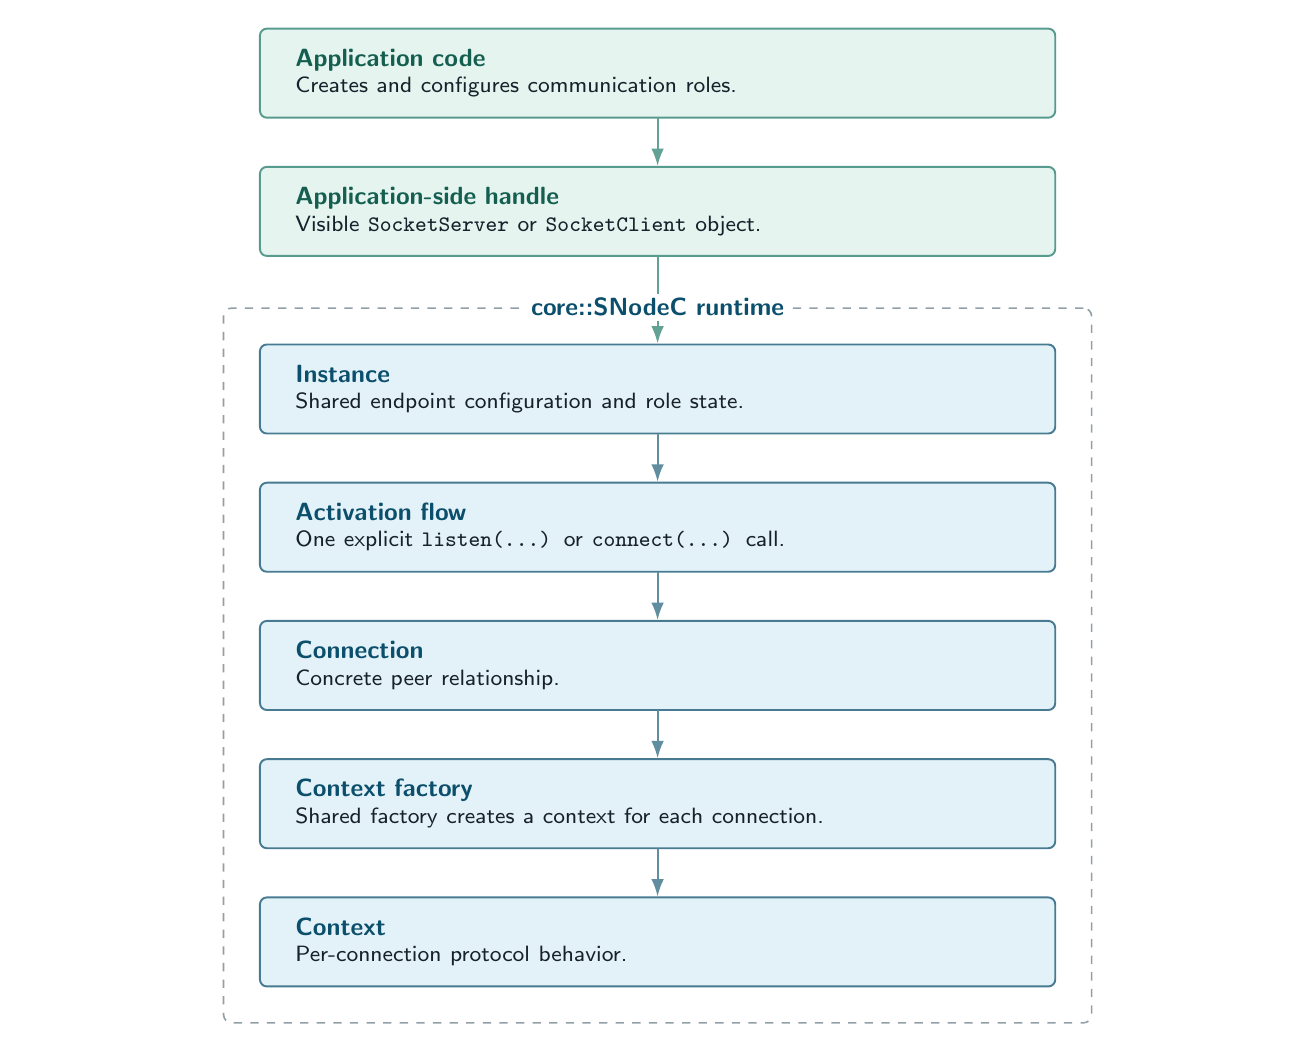
\begin{tikzpicture}[
  snodec diagram,
  app block/.style={
    draw=snodecGreen!75,
    fill=snodecGreenSoft,
    rounded corners=\snodecBoxCorner,
    line width=\snodecBoxLineWidth,
    align=left,
    text width=92mm,
    inner xsep=4.5mm,
    inner ysep=2.6mm,
    minimum height=11mm
  },
  runtime block/.style={
    draw=snodecBlue!75,
    fill=snodecBlueSoft,
    rounded corners=\snodecBoxCorner,
    line width=\snodecBoxLineWidth,
    align=left,
    text width=92mm,
    inner xsep=4.5mm,
    inner ysep=2.6mm,
    minimum height=11mm
  },
  flow/.style={snodec main arrow, draw=snodecBlue!65},
  register flow/.style={snodec main arrow, draw=snodecGreen!70},
  arrow label/.style={snodec arrow label}
]

\node[app block] (appcode) {\textbf{\textcolor{snodecTitleGreen}{Application code}}\\[-0.5mm]
  {\footnotesize Creates and configures communication roles.}
};

\node[app block, below=\snodecGapSmall of appcode] (handle) {\textbf{\textcolor{snodecTitleGreen}{Application-side handle}}\\[-0.5mm]
  {\footnotesize Visible \texttt{SocketServer} or \texttt{SocketClient} object.}
};

\node[runtime block, below=\snodecGapLarge of handle] (instance) {\textbf{\textcolor{snodecTitleBlue}{Instance}}\\[-0.5mm]
  {\footnotesize Shared endpoint configuration and role state.}
};

\node[runtime block, below=\snodecGapSmall of instance] (activation) {\textbf{\textcolor{snodecTitleBlue}{Activation flow}}\\[-0.5mm]
  {\footnotesize One explicit \texttt{listen(...)} or \texttt{connect(...)} call.}
};

\node[runtime block, below=\snodecGapSmall of activation] (connection) {\textbf{\textcolor{snodecTitleBlue}{Connection}}\\[-0.5mm]
  {\footnotesize Concrete peer relationship.}
};

\node[runtime block, below=\snodecGapSmall of connection] (factory) {\textbf{\textcolor{snodecTitleBlue}{Context factory}}\\[-0.5mm]
  {\footnotesize Shared factory creates a context for each connection.}
};

\node[runtime block, below=\snodecGapSmall of factory] (context) {\textbf{\textcolor{snodecTitleBlue}{Context}}\\[-0.5mm]
  {\footnotesize Per-connection protocol behavior.}
};

\draw[register flow] (appcode.south) -- (handle.north);
\draw[register flow] (handle.south) -- (instance.north);
\draw[flow] (instance.south) -- (activation.north);
\draw[flow] (activation.south) -- (connection.north);
\draw[flow] (connection.south) -- (factory.north);
\draw[flow] (factory.south) -- (context.north);

\begin{scope}[on background layer]
  \node[
    fit=(instance)(connection)(factory)(context),
    snodec boundary,
    inner sep=\snodecBoundaryInnerSep
  ] (runtime) {};
\end{scope}

% Foreground overlay title: masks the dashed border and any arrow below it.

\node[snodec boundary title] at (runtime.north) {core::SNodeC runtime};

\snodecApplyFixedCanvas

\end{tikzpicture}
\end{document}
